% ****** Start of file apssamp.tex ******
%
%   This file is part of the APS files in the REVTeX 4.2 distribution.
%   Version 4.2a of REVTeX, December 2014
%
%   Copyright (c) 2014 The American Physical Society.
%
%   See the REVTeX 4 README file for restrictions and more information.
%
% TeX'ing this file requires that you have AMS-LaTeX 2.0 installed
% as well as the rest of the prerequisites for REVTeX 4.2
%
% See the REVTeX 4 README file
% It also requires running BibTeX. The commands are as follows:
%
%  1)  latex apssamp.tex
%  2)  bibtex apssamp
%  3)  latex apssamp.tex
%  4)  latex apssamp.tex
%
\documentclass[%
 reprint,
%superscriptaddress,
%groupedaddress,
%unsortedaddress,
%runinaddress,
%frontmatterverbose, 
%preprint,
%preprintnumbers,
%nofootinbib,
%nobibnotes,
%bibnotes,
 amsmath,amssymb,
 aps,
%pra,
%prb,
%rmp,
%prstab,
%prstper,
%floatfix,
]{revtex4-2}

\usepackage{graphicx}% Include figure files
\usepackage{dcolumn}% Align table columns on decimal point
\usepackage{bm}% bold math
%\usepackage{hyperref}% add hypertext capabilities
%\usepackage[mathlines]{lineno}% Enable numbering of text and display math
%\linenumbers\relax % Commence numbering lines

%\usepackage[showframe,%Uncomment any one of the following lines to test 
%%scale=0.7, marginratio={1:1, 2:3}, ignoreall,% default settings
%%text={7in,10in},centering,
%%margin=1.5in,
%%total={6.5in,8.75in}, top=1.2in, left=0.9in, includefoot,
%%height=10in,a5paper,hmargin={3cm,0.8in},
%]{geometry}

\begin{document}

\preprint{APS/123-QED}

\title{Predicting Roll-Call Vote in the U.S Senate \\ A Neural Network Approach}% Force line breaks with \\

\author{David M. Thuman}
\email{dmt93@cornell.edu}
\affiliation{PHYS 4410 \\ Applied and Engineering Physics, Cornell University}

\date{\today}% It is always \today, today,
             %  but any date may be explicitly specified

\begin{abstract}
In this report, I will break the main components and hyperparameters that go into designing, building, and training a neural network. Once these components are broken down, I will use the knowledge gained to implement a neural network that predicts the roll-call votes of Senator Patrick Leahy using text features extracted from the legislature the votes are based on. In the end, a network was created that out-performed the baseline of Always-Yes.
\end{abstract}

%\keywords{Suggested keywords}%Use showkeys class option if keyword
                              %display desired
\maketitle

%\tableofcontents

\section{Introduction}

When viewing Google Trend's data on words like 'ML', 'AI', 'Machine Learning', and 'Neural Network', a picture is painted of increased interest in the field of artificial intelligence. At this point in time, most large-scale companies have some type of AI model working to help solve their problems.

Moreover, as more and more data is being created, collected, and processed, the information that can be assessed when looking to solve a problem is incalculable. Handling that much data becomes too hard of a problem for a human to do.

This is when we look to computers to help solve this problem-solving problem.

\subsection{Neural Networks}

Simply put, all a neural network does is matrix multiplication and addition. This idea of "learing", in a general sense, is created through complexity; emergent properties of a system are only evident when components are combined. So let us take a small tour of these components.

\subsubsection{Neuron}

At a high level, a neuron is a function; it takes in a set of inputs, does calculations based on its internal parameters, and produces an output.

These internal parameters, which will make more sense in the context of combining neurons together, are the input weights, the neuron bias, and the activation function. For a single neuron, its calculation might look like

\begin{equation*}
    output = ActiveFunc \bigg (\sum_k w_k*input_k + bias \bigg)
\end{equation*}

All the $k$ inputs are multiplied by their weight and summed together. A bias is then added to adjust the sum's relation to zero, which is then run through an activation function to produce an output that is between 0 and 1. 

\subsubsection{Architecture}

To gain this complexity, neurons are combined into layers that do not connect to each other. Layers are then combined sequentially. The input layer is connected to the hidden layers, which are then connected to the output layer. Every neuron in one layer is connected to every other neuron in the next layer.

Once this network is built, all the connection weights and neuron biases are the network parameters. These will be the numbers that are tuned when the neural network is trained.

\subsubsection{Training}

The one goal for a neural network is to correctly predict a classification given an input set. And with any goal, there need to be some methods to measure success and failure. Loss Functions are used to compare the target output with the predicted one. During training, the end goal is to minimize the network's loss function.

To tune the network parameters mentioned above in order to decrease the loss function, an algorithm called backpropagation is used. It determines how a single training example should nudge the network parameters.

As the goal during training is to decrease the loss function, a gradient of the loss function (the direction of largest change) in the parameter space (a vector of how much the loss function changes for each weight and bias) must be calculated. This derivative of the loss function with respect to each parameter cannot be calculated directly, so the chain rule is used to calculate these partial derivatives\cite{Nielsen}.

As the backpropagation algorithm is not the focus of this report, the detailed mathematics will not be discussed further than this.

\subsection{Roll-Call Votes}

In the realm of quantitative political science, building models using the rich data set of legislative roll-call votes seems to be everyone's starting point\cite{Goldblatt2012HowAB}. And the same goes for this paper.

In Congress, roll-call votes are the only votes for which a public record is made of how individual members of Congress voted. Few bills actually receive a roll-call vote, which can be for the passing of a piece of legislature, amendments, nominations, motions, or cloture motions.

The goal of this report is to build a neural network to predict a vote for a single Senator, given a bill. As we cannot place the whole of the bill as the input to a neural network, some form of data processing will occur on the text of the bill in an attempt to extract some "meaning".

Being able to predict the roll-call votes for a given bill has no direct applications. However, practicing one's modeling skills within the political realm will help to push quantitative political science to better models and hopefully better theories.

\section{Data Preparation}

To keep the paper's focus small, a single model was created to predict the roll-call vote of Senator Patrick Leahy (D-VT). The specific choice of Senator Leahy was one of data abundance. Leahy was first elected to the Senate in 1974 and is currently in his 8th term. Therefore, the data available for a single-Senator model was most robust for Senator Leahy.

The goal is to prepare 4 different feature mapping for all of the bills. The first is a unigram binary feature, which takes the top 4000 highest ranking unigrams (single words) based on their Term Frequency - Inverse Document Frequency (TF-IDF). This list is then used to create the bill's input, seeing whether that unigram is contained in the bill's text or not. TF-IDF is a common natural language processing (NLP) calculation to extract relevant words from a corpus or series of documents. Words are ranked highly if they are very frequent throughout all the bills and punished for being contained in a higher amount of bills. This same process is done on bigrams (two-word phrases) to create all the bill's bigram binary features.

Using the same top-ranked 4000 unigrams and bigrams, a bag-of-words feature is also used instead of a binary. For these features, counts of how many times that unigram or bigram appears in a bill's text is used as the input.

\subsection{Data Collection}

Roll-call votes from the 101st to the 117th Congress were pulled from senate.gov\cite{senate}. Of these votes, only the ones that were on the passage of the bill and where Senator Leahy made a vote were kept. Roll-call votes with regard to the passage of a bill appear to be the minority of votes taken, so only 594 votes were taken. The choice to only pick roll-call votes for the passage of the bill was because this vote has the most direct relation to the bill's text, while votes on motions and cloture motions can be less related to the text. Once a vote was found, its associated bill was pulled from congress.gov\cite{congress}.

\subsection{Data Cleaning}

As an NLP model is not being utilized to extract "meaning" from the bill's text, data cleaning and pre-processing are extremely important as it allows our input features to informative and consistent. Words like 'the', 'and', or 'of' are extremely common in the English language, but carry little to no meaning when looking at the corpus of a bill. These zero-meaning words are commonly referred to as stop-words. To clear all the bills of these stop-words, two sets of words were taken. One is the top 100 most frequent words in the English language\cite{unigram}, and the second is a list of stop-words from an outside resource\cite{stop}. All of these words are then removed from each bill. Please note that although we are changing the wording of the bills, the grammatical structure is not pulled as a feature for the neural network, so no substantial change has occurred.

\subsection{Data Processing}

As stated above, once all the bills have been cleaned, the top-ranked 4000 unigrams and bigrams can be found from all the bills. Once these lists have been created, we are able to create inputs for all the bills, for all four of the different feature types: unigram binary, bigram binary, unigram bag, and bigram bag.

Train-Test splits are then created for all four data features. The test size was set to 15\% of the total data collected, and the split is stratified on the output so that the ratio of 'Yeas' to 'Nays' is equivalent between the training data and the testing data. This is done because the voting data for Senator Leahy is heavily biased to 'Yes'.

\section{Neural Network Model}

Data preparation is only half the problem; designing the architecture of the neural network, specifically picking the hyperparameters of the neural network, is a whole other problem. In general, there are no hard-and-fast rules for picking the hyperparameters for a neural network. There is, of course, some guidance when the specific problem that the neural network is decided on (in our case this is a Binary Classification problem).

\subsection{Hyperparameters}

Hyperparameters are aspects of the neural network that are not tuned or optimized during the training of the network. These are architectural choices that help to fully optimize the network.

\subsubsection{Hidden Layers}

From the quick introduction of neural networks above, hidden layers are layers of neurons that are placed in between the input layer and the output layer. There are two main questions that come up when discussing hidden layers: How many units (neurons) should be within a layer? How many hidden layers should be added?

For how many units, the general consensus is that the number of neurons in the hidden layer should be between the number of units of its two adjacent layers.

For the number of hidden layers, again the general consensus is that most problems can be solved with only a single hidden layer.

For this neuron network, a single hidden layer was added. Moreover, because our input layer has 4000 units and our output layer has 1 neuron, this hidden layer will have 2000 units.

\subsubsection{Optimizer}

During the brief overview of backpropagation, it was stated that the gradient of the loss function was needed to tune all the weights and biases of the network. The true gradient of the loss function is found when we average over the gradient vectors for all the training examples. For large data sets, this is computationally expensive and timely, so different optimization algorithms have been created to help solve this problem.

Two optimizers were tested when exploring different network architectures: Stochastic Gradient Descent (SGD), and Adaptive Moment Estimation (ADAM). In the end, ADAM was chosen as it had the highest performance when decreasing the loss function.




Another choice when deciding on an optimizer setup is its learning rate. When the optimizer is calculating the loss function's gradient, at a high level it is attempting to find a local or the global minimum of the function. Every time a gradient is calculated and the parameters are updated, a step is taken downhill towards the loss functions minimum. The size of this step is dependent on the learning rate of the optimizer. A larger learning rate allows the optimizer to decrease the loss function with fewer iterations but might have an unintended effect of overshooting the minimum and therefore increasing the loss function. A smaller learning rate will allow the optimizer to make more precise steps but will take more iterations to converge.

Through trial-and-error and online resources, a learning rate of 0.0001 was chosen.

\subsubsection{Loss Function}

The loss function of the network quantitatively tells how well the network is predicting when compared to the target output. Unlike some choices for hyperparameters, different loss functions have been created for specific problems.

In our case, because we are attempting to a binary choice, our problem is a Binary Classification problem. With this type of problem, all the literature points to using the Binary Cross Entropy loss function.

\begin{equation*}
    H_p(q) = -\frac{1}{N}\sum_{i=1}^N y_i \log(p(y_i)) + (1-y_i) \log(1-p(y_i))
\end{equation*}

\subsubsection{Activation Functions}

Activation functions for neurons mimic the way a neuron in the brain can be 'on' or 'off', 'active' or 'inactive'.  Because a neuron's activation is a summation of all its inputs times their weights plus a bias, this number is likely not between 0 and 1. To map the number to a value between 0 and 1, different activation functions are assigned to neurons on a per-layer basis.

The input layer to a network does not need an activation function as your input features should be already set. For hidden layers, the best training results are shown from rectified linear functions. The function can be seen below.

\begin{equation*}
    ReLu(z) = max\{0, z\}
\end{equation*}

The activation function for the output layer is in general also connected to the type of problem you are solving. In this case, a sigmoid or hard sigmoid are the best for the problem, and through testing, the sigmoid 
the function was chosen for its improved total accuracy.

\begin{equation*}
    S(z) = \frac{1}{1 + e^{-x}}
\end{equation*}

\subsubsection{Number of Epochs and Batch Size}

Training neural networks is an iterative process. The number of epochs determines how many total iterations occur over all the training data. Multiple runs over the training data allow the loss function to converge on a number.

As stated in the optimizer section, often times it is too computationally expensive to calculate the true gradient of the loss function. Batches are equal subsets of the total training data that are used to calculate an approximate gradient.

A larger batch size gives a better gradient to tune the parameters, and through trial-and-error, 200, or around half to one-third of the training set.

The number of epochs heavily depends on your learning rate. If your learning rate is low, you will need more steps (iterations) over the training data to converge to a local or global minimum of the loss function.

\section{Results}

After testing out many different hyperparameter combinations, I was able to maximize the accuracy of the 4 different feature sets to differing amounts above the standard baseline of an Always-Yes predictive model.

\begin{table}[h!]
\centering
\begin{tabular}{|p{0.10\textwidth}|p{0.15\textwidth}|p{0.09\textwidth}|p{0.10\textwidth}|} 
 \hline
 \textbf{N-gram} & \textbf{Features} & \textbf{Loss} & \textbf{Accuracy} \\
 \hline
 \hline
 - & Always-Yes & - & 0.823 \\ 
 \hline
 Unigram & Binary & 0.419 & 0.833 \\ 
 \hline
 Bigrma & Binary & 0.353 & 0.889 \\ 
 \hline
 Unigram & Bag-of-Words & 1.860 & 0.833 \\ 
 \hline
 Bigram & Bag-of-Words & 0.904 & 0.844 \\ 
 \hline
 \end{tabular}
\caption{\label{tab:table-name} Five different data models with their loss and accuracy values. The neural network has an input layer of 4000 units, a single hidden layer of 2000 units, and an output layer of 1 unit.}
\end{table}

As we can see, the bigram binary feature has the best predictive accuracy out of the 4 data models.

We can also look into the training and validation accuracy as a function of the number of epochs which can be seen in Figure 1.

\begin{figure}
    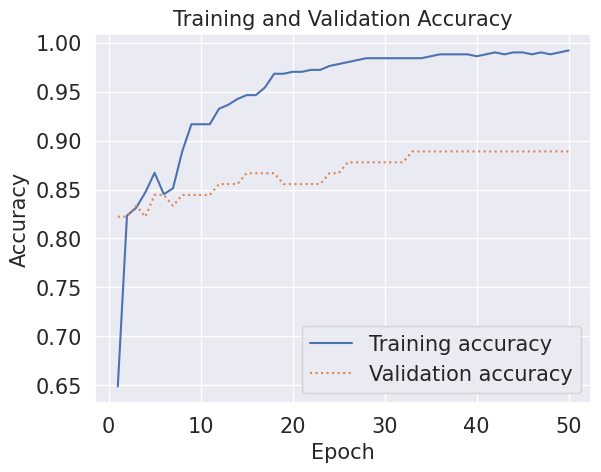
\includegraphics[width=0.48\textwidth]{bigram_binary_acc.png}
    \caption{Training and Validation Accuracy for the Bigram Binary feature set. The learning rate for the neural network is set to 0.0001 with a batch size of 200.}
\end{figure}

Looking at Figure 1, we can see convergence for both the training and the validation accuracy as more training occurs. However, this gap between the training and validation curves is a product of overfitting the neural network on the training set.

Figure 2 shows a precision matrix that allows us to take a look inside the model to see what prediction it is making.

\begin{figure}
    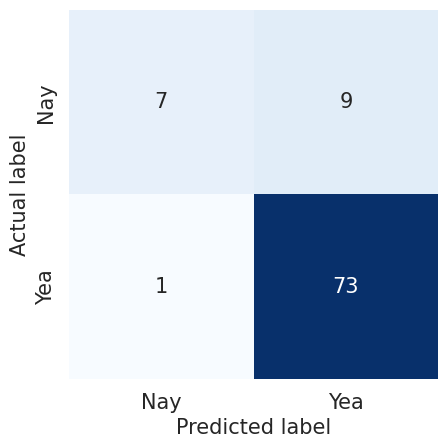
\includegraphics[width=0.40\textwidth]{bigram_binary_grid.png}
    \caption{A Precision Matrix for the Bigram Binary feature set. The matrix shows how the neural network is correctly and incorrectly predicting votes for a target 'Yea' and 'Nay'.}
\end{figure}

As we can see, the data set is heavily biased towards 'Yeas'. However, the neural network is still able to learn above the accuracy of a naive Always-Yes.

\subsection{Overfitting}

A clear sin of overfitting in a model is the gap between the training accuracy and the validation accuracy. Overfitting can occur when the total size of the data set is small or if the input features are too large or complex. With regards to this model, data features using only the top 1000 unigrams and bigrams were also tested with the same result. Moreover, with a total data set of around 600 examples, a large portion of the overfitting problem most likely occurs from the lack of a large data set.

\section{Future Work}

It is clear that improvements can be made to this predictive model. First, the cleaning, picking, and building of the data features are not very involved. Simple decisions are made to build a simple NLP model in the front. If improvements were to be made, an actual natural language process model may be utilized to pull more "meaningful" text data from the bills.

Another improvement that would be necessary in the future is to increase the size of the data set. In general, more training examples for the network will result in better performance. Moreover, the clear overfitting problem would be decreased if more data were available to train on.

\section{Conclusion}

This report set out to accomplish two goals: to predict roll-call votes in Congress using the text from its legislature and to gain the skills necessary to confidently design, build, and train a neural network to complete the first goal.

\appendix

\section{Code}

Here is the link to the Github reposotory \url{https://github.com/davidthuman/Roll-Call-Predictor}

% The \nocite command causes all entries in a bibliography to be printed out
% whether or not they are actually referenced in the text. This is appropriate
% for the sample file to show the different styles of references, but authors
% most likely will not want to use it.
\nocite{*}

\bibliography{refs}% Produces the bibliography via BibTeX.

\end{document}
%
% ****** End of file apssamp.tex ******
